%%%%%%%%%%%%%%%%%%%%%%%%%%%%%%%%%%%%%%%%%
% Masters/Doctoral Thesis 
% LaTeX Template
% Version 2.5 (27/8/17)
%
% This template was downloaded from:
% http://www.LaTeXTemplates.com
%
% Version 2.x major modifications by:
% Vel (vel@latextemplates.com)
%
% This template is based on a template by:
% Steve Gunn (http://users.ecs.soton.ac.uk/srg/softwaretools/document/templates/)
% Sunil Patel (http://www.sunilpatel.co.uk/thesis-template/)
%
% Template license:
% CC BY-NC-SA 3.0 (http://creativecommons.org/licenses/by-nc-sa/3.0/)
%
%%%%%%%%%%%%%%%%%%%%%%%%%%%%%%%%%%%%%%%%%

%----------------------------------------------------------------------------------------
%	PACKAGES AND OTHER DOCUMENT CONFIGURATIONS
%----------------------------------------------------------------------------------------

\documentclass[
11pt, % The default document font size, options: 10pt, 11pt, 12pt
%oneside, % Two side (alternating margins) for binding by default, uncomment to switch to one side
english, % ngerman for German
singlespacing, % Single line spacing, alternatives: onehalfspacing or doublespacing
%draft, % Uncomment to enable draft mode (no pictures, no links, overfull hboxes indicated)
%nolistspacing, % If the document is onehalfspacing or doublespacing, uncomment this to set spacing in lists to single
liststotoc, % Uncomment to add the list of figures/tables/etc to the table of contents
toctotoc, % Uncomment to add the main table of contents to the table of contents
%parskip, % Uncomment to add space between paragraphs
%nohyperref, % Uncomment to not load the hyperref package
headsepline, % Uncomment to get a line under the header
%chapterinoneline, % Uncomment to place the chapter title next to the number on one line
consistentlayout, % Uncomment to change the layout of the declaration, abstract and acknowledgements pages to match the default layout
]{MastersDoctoralThesis} % The class file specifying the document structure

\usepackage[utf8]{inputenc} % Required for inputting international characters
\usepackage[T1]{fontenc} % Output font encoding for international characters

\usepackage{mathpazo} % Use the Palatino font by default

\usepackage[backend=bibtex,style=authoryear,natbib=true]{biblatex} % Use the bibtex backend with the authoryear citation style (which resembles APA)

\addbibresource{bibliography.bib} % The filename of the bibliography

\usepackage[autostyle=true]{csquotes} % Required to generate language-dependent quotes in the bibliography

%----------------------------------------------------------------------------------------
%	MARGIN SETTINGS
%----------------------------------------------------------------------------------------

\geometry{
	paper=a4paper, % Change to letterpaper for US letter
	inner=2.5cm, % Inner margin
	outer=3.8cm, % Outer margin
	bindingoffset=.5cm, % Binding offset
	top=1.5cm, % Top margin
	bottom=1.5cm, % Bottom margin
	%showframe, % Uncomment to show how the type block is set on the page
}

%----------------------------------------------------------------------------------------
%	THESIS INFORMATION
%----------------------------------------------------------------------------------------

\thesistitle{SLAM for Autonomous Planetary Exploration using Global Map Matching} % Your thesis title, this is used in the title and abstract, print it elsewhere with \ttitle
\supervisor{Assoc. Prof.\\ Loukas \textsc{Petrou}} % Your supervisor's name, this is used in the title page, print it elsewhere with \supname
\examiner{} % Your examiner's name, this is not currently used anywhere in the template, print it elsewhere with \examname
\degree{Diploma in Electrical and Computer Engineering} % Your degree name, this is used in the title page and abstract, print it elsewhere with \degreename
\author{Dimitrios \textsc{Geromichalos}} % Your name, this is used in the title page and abstract, print it elsewhere with \authorname
\addresses{} % Your address, this is not currently used anywhere in the template, print it elsewhere with \addressname

\subject{} % Your subject area, this is not currently used anywhere in the template, print it elsewhere with \subjectname
\keywords{} % Keywords for your thesis, this is not currently used anywhere in the template, print it elsewhere with \keywordnames
\university{Aristotle University of Thessaloniki} % Your university's name and URL, this is used in the title page and abstract, print it elsewhere with \univname
\department{School of Electrical and Computer Engineering} % Your department's name and URL, this is used in the title page and abstract, print it elsewhere with \deptname
\group{Research Group Name} % Your research group's name and URL, this is used in the title page, print it elsewhere with \groupname
\faculty{Faculty of Engineering} % Your faculty's name and URL, this is used in the title page and abstract, print it elsewhere with \facname

\AtBeginDocument{
\hypersetup{pdftitle=\ttitle} % Set the PDF's title to your title
\hypersetup{pdfauthor=\authorname} % Set the PDF's author to your name
\hypersetup{pdfkeywords=\keywordnames} % Set the PDF's keywords to your keywords
}

\begin{document}

\frontmatter % Use roman page numbering style (i, ii, iii, iv...) for the pre-content pages

\pagestyle{plain} % Default to the plain heading style until the thesis style is called for the body content

%----------------------------------------------------------------------------------------
%	TITLE PAGE
%----------------------------------------------------------------------------------------

\begin{titlepage}
\begin{center}

\vspace*{.06\textheight}
{\scshape\LARGE \univname\par}\vspace{2.5cm} % University name
% \textsc{\Large Diploma Thesis}\\[0.5cm] % Thesis type

\HRule \\[0.4cm] % Horizontal line
{\huge \bfseries \ttitle\par}\vspace{0.4cm} % Thesis title
\HRule \\[2.5cm] % Horizontal line
 
\begin{minipage}[t]{0.4\textwidth}
\begin{flushleft} \large
\emph{Author:}\\ {\authorname} % Author name - remove the \href bracket to remove the link
\end{flushleft}
\end{minipage}
\begin{minipage}[t]{0.4\textwidth}
\begin{flushright} \large
\emph{Supervisor:} \\ {\supname} % Supervisor name - remove the \href bracket to remove the link  
\end{flushright}
\end{minipage}\\[3cm]
 
\vfill

\large \textit{A dissertation submitted to the \facname\\ in partial fulfillment of the requirements for the degree of}\\[0.3cm] % University requirement text
Diploma\\in\\Electrical and Computer Engineering\\[2cm]
% \deptname\\[2cm] % Research group name and department name
% \textit{in}\\[0.4cm]
% \deptname\\[2cm] % Research group name and department name
 
\vfill

{\large \today\\Thessaloniki, Greece}\\[4cm] % Date
%\includegraphics{Logo} % University/department logo - uncomment to place it
 
\vfill
\end{center}
\end{titlepage}

%----------------------------------------------------------------------------------------
%	DECLARATION PAGE
%----------------------------------------------------------------------------------------

% \begin{declaration}
% \addchaptertocentry{\authorshipname} % Add the declaration to the table of contents
% \noindent I, \authorname, declare that this thesis titled, \enquote{\ttitle} and the work presented in it are my own. I confirm that:

% \begin{itemize} 
% \item This work was done wholly or mainly while in candidature for a research degree at this University.
% \item Where any part of this thesis has previously been submitted for a degree or any other qualification at this University or any other institution, this has been clearly stated.
% \item Where I have consulted the published work of others, this is always clearly attributed.
% \item Where I have quoted from the work of others, the source is always given. With the exception of such quotations, this thesis is entirely my own work.
% \item I have acknowledged all main sources of help.
% \item Where the thesis is based on work done by myself jointly with others, I have made clear exactly what was done by others and what I have contributed myself.
% \end{itemize}
 
% \noindent Signed:\\
% \rule[0.5em]{25em}{0.5pt} % This prints a line for the signature
 
% \noindent Date:\\
% \rule[0.5em]{25em}{0.5pt} % This prints a line to write the date
% \end{declaration}

% \cleardoublepage

%----------------------------------------------------------------------------------------
%	QUOTATION PAGE
%----------------------------------------------------------------------------------------

% \vspace*{0.2\textheight}

% \noindent\enquote{\itshape Thanks to my solid academic training, today I can write hundreds of words on virtually any topic without possessing a shred of information, which is how I got a good job in journalism.}\bigbreak

% \hfill Dave Barry

%----------------------------------------------------------------------------------------
%	ABSTRACT PAGE
%----------------------------------------------------------------------------------------

\begin{abstract}
\addchaptertocentry{\abstractname} % Add the abstract to the table of contents
Write abstract here...\ldots
\end{abstract}

%----------------------------------------------------------------------------------------
%	ACKNOWLEDGEMENTS
%----------------------------------------------------------------------------------------

% \begin{acknowledgements}
% \addchaptertocentry{\acknowledgementname} % Add the acknowledgements to the table of contents
% The acknowledgments and the people to thank go here, don't forget to include your project advisor\ldots
% \end{acknowledgements}

%----------------------------------------------------------------------------------------
%	LIST OF CONTENTS/FIGURES/TABLES PAGES
%----------------------------------------------------------------------------------------

\tableofcontents % Prints the main table of contents

\listoffigures % Prints the list of figures

\listoftables % Prints the list of tables

%----------------------------------------------------------------------------------------
%	ABBREVIATIONS
%----------------------------------------------------------------------------------------

%\begin{abbreviations}{ll} % Include a list of abbreviations (a table of two columns)

%\textbf{LAH} & \textbf{L}ist \textbf{A}bbreviations \textbf{H}ere\\
%\textbf{WSF} & \textbf{W}hat (it) \textbf{S}tands \textbf{F}or\\

%\end{abbreviations}

%----------------------------------------------------------------------------------------
%	PHYSICAL CONSTANTS/OTHER DEFINITIONS
%----------------------------------------------------------------------------------------

%\begin{constants}{lr@{${}={}$}l} % The list of physical constants is a three column table

% The \SI{}{} command is provided by the siunitx package, see its documentation for instructions on how to use it

%Speed of Light & $c_{0}$ & \SI{2.99792458e8}{\meter\per\second} (exact)\\
%Constant Name & $Symbol$ & $Constant Value$ with units\\

%\end{constants}

%----------------------------------------------------------------------------------------
%	SYMBOLS
%----------------------------------------------------------------------------------------

% \begin{symbols}{lll} % Include a list of Symbols (a three column table)

% $a$ & distance & \si{\meter} \\
% $P$ & power & \si{\watt} (\si{\joule\per\second}) \\
%Symbol & Name & Unit \\

% \addlinespace % Gap to separate the Roman symbols from the Greek

% $\omega$ & angular frequency & \si{\radian} \\

% \end{symbols}

%----------------------------------------------------------------------------------------
%	DEDICATION
%----------------------------------------------------------------------------------------

% \dedicatory{For/Dedicated to/To my\ldots} 

%----------------------------------------------------------------------------------------
%	THESIS CONTENT - CHAPTERS
%----------------------------------------------------------------------------------------

\mainmatter % Begin numeric (1,2,3...) page numbering

\pagestyle{thesis} % Return the page headers back to the "thesis" style

% Include the chapters of the thesis as separate files from the Chapters folder
% Uncomment the lines as you write the chapters

\label{Chapter1}

\chapter{Introduction}

\section{Motivation}

Mention the scope, its state, the current issues and what is needed to
solve them

\begin{itemize}
    \item Scope: planetary exploration (for scientific purposes)
    \item State: past and current missions, their purpose and outcome/state
    \item Issues: no constant communication, manual command sequence, unsafe/upredictable conditions
    \item Needed: real-time and low-supervision system/platform
\end{itemize}

\section{Problem Statement}

Mention the environment and the robot's equipment and purpose\\
Mention that the problem is given X inputs to calculate Y outputs

\begin{itemize}
    \item Environment: extreme planetary terrains with anomalies (rocks and craters) and high elevation variance
    \item Equipment: mechanical and sensor configuration
    \item Purpose: autonomous (low-supervision) navigation
    \item Inputs: odometry pose, sensor inputs, imu, global map
    \item Outputs: corrected pose, local elevation map
\end{itemize}

\subsection{Presumptions}

Explain what presumptions are made to the problem

\begin{itemize}
    \item Initial global position is known
    \item Environment is static (not true for autonomous driving applications of algorithm)
    \item Environment is unknown (no high resolution a priori maps) (not true for autonomous driving applications of algorithm)
    \item Terrain is single layered (no bridges etc.)
\end{itemize}

\section{Literature Review}

\subsection{SLAM}

\begin{itemize}
    \item  What is SLAM
        \begin{itemize}
            \item typical explanation in literature
            \item categories
        \end{itemize}
    \item How is SLAM implemented
        \begin{itemize}
            \item volumetric/feature based approaches
            \item grid-based fast slam
            \item etc. etc. etc.
        \end{itemize}
\end{itemize}

\subsection{Planetary Absolute Localization}

Mention how is absolute localization achieved in planetary applications

\begin{itemize}
    \item Feature based approaches
    \item Skyline based approaches
    \item map based approaches
\end{itemize}

\section{Thesis Objectives and Organization}

\subsection{Research Objectives}

Mention what are the main objectives in terms of research

\begin{itemize}
    \item Develop a novel technique for minimizing drift in global localization with global map matching and an execution strategy (criteria)
    \item Determine under what circumstances (i.e. resolution, local and global) can the orbital imagery be useful for SLAM
    \item Examine and quantify the gains (better localization, by providing a navigable map with the resolution and dense distribution restrictions that come with it) and loses (processing overhead)
\end{itemize}

\subsection{Organization}

Explain how this thesis is structured


%\label{Chapter2}

\chapter{System Architecture}

\section{System Overview} \label{system_overview}

In order for planetary robots to navigate autonomously in extreme and
uncertain conditions where no GPS information is available,
they need to perceive their surroundings with high precision and
maintain this precision over time.
A way of compensating for the lack of real-time GPS data, is to use
an \textit{a priori} global map that contains 3D information about the
environment the robot is trying to navigate into.
This map can be reconstructed using imagery taken from an orbiter and
has a notably lower resolution compared to the robot's sensory data.
To take advantage of this existing information, we have developed a system
which is based around two layers of data processing.

In the first tier, the objective is to perceive the environment and
capture its 3D structure so as to enable the robot to navigate in it.
This is achieved by constructing a local map and estimating the robot's
current pose (position and orientation) w.r.t. its initial pose,
using sensory inputs and odometry data.
This process is commonly known as
\textit{Simultaneous Localization And Mapping} (SLAM) and can be expressed as
\begin{equation}
    p(x_{0:T} ,\ m_{1:T} \ | \ z_{1:T} ,\ u_{1:T})
\end{equation}
where
$x$ are the estimated poses of the robot,
$m$ is the constructed map of the environment,
$z$ are the sensory inputs and
$u$ are the robot's controls.
To reduce the problem's dimensions, the following factorization is performed
\begin{equation}
    p(x_{0:T} ,\ m_{1:T} \ | \ z_{1:T} ,\ u_{1:T}) =
    p(x_{0:T} \ | \ m_{1:T-1} ,\ z_{1:T} ,\ u_{1:T}) \
    p(m_{1:T} \ | \ x_{0:T} ,\ z_{1:T})
\end{equation}
where
the former belief represents the pose estimation problem, also called
relative localization, and the latter belief represents the mapping problem.

In the second tier, the objective is to achieve absolute localization by
eliminating the accumulated drift which occurs in the previous stage.
This drift is present in long-range scenarios and comes from the fact that
all the input information is coming directly from the robot itself.
To eliminate it, a matching technique is utilized with the aim of finding the
position of the robot's local map inside a global map.

The separation of the system to two layers comes from the need to process the
data in separate moments, depending on the conditions of the environment as
well as on the robot's processing capabilities.
In Figure \ref{fig:HLD}, the high-level design diagram of the system shows
the 4 main modules that comprise the entire system.
Their functionality is explained in the following sections of this chapter.

\begin{figure}[th]
    \centering
    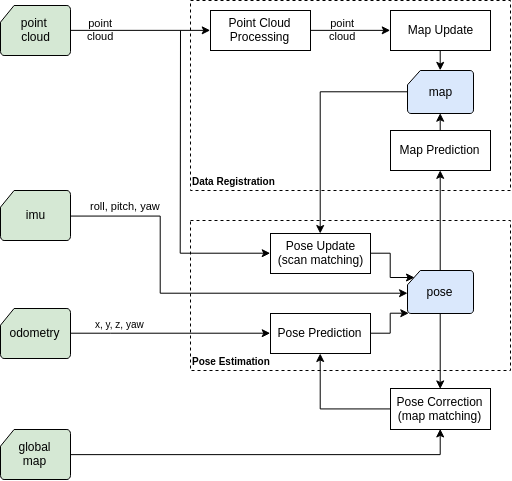
\includegraphics[scale=0.4]{Figures/high_level_design_diagram}
    \decoRule
    \caption[High Level Design Diagram]{
        The high-level design diagram showing the submodules that comprise
        the system as well as the data flow.}
    \label{fig:HLD}
\end{figure}

\section{Data Registration}

An integral aspect of a robotic system, is the mapping process.
In the previous chapter (Section \ref{system_overview}) this processed
was expressed as
\begin{equation}
    p(m_{1:T} \ | \ x_{0:T} ,\ z_{1:T})
\end{equation}
where
$m$ is the posterior map of the environment,
$x$ are the estimated poses of the robot and
$z$ are the sensory inputs.
The map is the model of the environment and can represent information about
it in either two or three dimensions.
In addition, the information a map represents can be organized either in
a grid-based manner (volumetric map) or in the form of landmarks
(feature-based map).
Volumetric maps provide a more detailed and precise model of the environment
compared to feature-based maps and are, therefore, the better choice for
robots that aim to solve navigation tasks.
Moreover, autonomous robots that need to navigate in non-flat surfaces,
require a 3D model as a means to safely avoid the terrain's obstacles.
Robotic applications with this requirement include outdoor, underwater,
airborne or planetary missions.

% TODO(ref): mapping and classification

As we have already mentioned, planetary rovers have an important constraint
in on-board computational power.
This limitation deems the use of pure 3D maps inappropriate.
To overcome this problem, we can represent the environment with a 2.5D map,
known as elevation map.
An elevation map is essentially a 2D grid-map composed of cells that hold
the value of the terrain's elevation.
It is important to note that this mapping method does not model completely
the 3D environment, but can provide a sufficient approximation even for
the most demanding applications.

% TODO(ref): elevation map

To make use of this mapping technique, a robot must be equipped with a
sensor that is capable of providing measurements in the 3D space.
Such measurements are usually stored in a structure called point cloud -
a set of points $P$ that contain information about their position in
space $(x,y,z)$.
A point cloud can be constructed from sensors that provide depth information,
with the most popular being stereo cameras, time-of-flight (ToF) cameras
and LiDARs.

% TODO(ref): point cloud

In this section, the functionality of the Data Registration module will be
explained.
Its main purpose is to preprocess the input sensor data (point cloud)
and register it to create an elevation map or update an existing one.

\subsection{Point Cloud Preprocessing} \label{point_cloud_processing}

The importance of preprocessing a point cloud before registering its data
in a map, comes from the fact that point clouds contain large amount of points
and hence process them is a time-consuming task.
Additionally, the points represented in the cloud may be referenced in a
different frame (usually the sensor's frame) than the frame of the map.

For this purpose, we implemented a point cloud preprocessing submodule,
that consists of the following four steps:

\begin{enumerate}
    \item \textbf{Voxelization}:
        In this step, we reduce the volume of the point cloud by downsampling
        it using a discrete 3D grid.
        Each cell of the grid, called \textit{voxel}, is mapped to $\{0,1\}$
        and it therefore represents the existence or absence of an obstacle
        in that position.
        This method is called \textit{voxelization} and results in a more
        sparse cloud of 3D points.
        % However, the larger the voxels are, the less precise the
        % representation of the space becomes.

        % TODO: Add equation for voxelization
        % TODO(ref): voxelization

    \item \textbf{Transformation}:
        A point $P$ sampled from the sensor is in the sensor's reference frame
        $S$ and need to be transformed in the map's frame $M$ in order to be
        registered.
        This is be achieved by
        \begin{equation}
            \mathbf{t}_{MP} =
                \mathbf{R}_{SM} \mathbf{t}_{SP} -
                \mathbf{t}_{SM}
        \end{equation}
        where
        $\mathbf{t}_{MP}$ is the position of $P$ in the map frame,
        $\mathbf{t}_{SP}$ is the position of $P$ in the sensor frame,
        $\mathbf{R}_{SM}$ is the rotation between the sensor frame and the
        map frame and
        $\mathbf{t}_{SM}$ is the translation between them.

    \item \textbf{Cropping}:
        Since a point cloud can span a wide area in space depending on the
        sensor's field of view and orientation, we can further reduce the
        volume of the cloud by discarding (cropping) points that fall out
        of the map.
        This is done by defining a box in space and removing
        from the point set all the points that are not inside it.
        In our case, we define the minimum and maximum cutoff points that
        represent the diagonal of the crop box as
        \begin{equation}
        \begin{aligned}
            &min\_cutoff\_point =
                \left( \
                    - \frac{l_x}{2} - t_x, \
                    - \frac{l_y}{2} - t_y, \
                    z_{min} \
                \right) \\
            &max\_cutoff\_point =
                \left( \
                    \frac{l_x}{2} + t_x, \
                    \frac{l_y}{2} + t_y, \
                    z_{max} \
                \right)
        \end{aligned}
        \end{equation}
        where
        $l_x$ and $l_y$ are the lengths of the map in meters in the
        x and y axis,
        $t_x$ and $t_y$ are the positions of the map in meters in the
        x and y axis and
        $z_{min}$ and $z_{max}$ are the minimum and maximum elevation
        of the map.

    \item \textbf{Uncertainty calculation}:
        In this last step, we use the sensor's model to calculate the variance
        of each point in the point cloud, $\sigma^2_z$.
        As a result, each point will contain in addition to a $x$ and $y$
        position, a one-dimensional Gaussian distribution for the height.
        This calculation is different for every sensor, since it depends
        on the sensor's characteristic.
        For a stereo camera, we approximate the variance as
        \begin{equation}
            \sigma^2_z = \dots
        \end{equation}
\end{enumerate}

% TODO: Add figure of point cloud pre and post processing

\subsection{Registration}

\subsubsection{Structure of Elevation Map} \label{map_structure}

The elevation map, also referred to as \textit{local map} or simply
\textit{map}, is a robot-centric grid-based map.
This means that it is centered in the robot's position in the
global reference frame.
When the robot moves, previous cells that now fall out of the map are
reset and values that belong to the new explored area take their place.

The map models the elevation of the environment as well as the uncertainty
of it.
As a result, in every position of the 2D grid, the elevation is
represented by a one-dimensional Gaussian distribution.
This means that the map consists of two layers

\begin{itemize}
    \item the layer of \textit{mean} elevation $(\mu_z)$ and
    \item the layer of elevation \textit{variance} $(\sigma^2_z)$
\end{itemize}
% TODO: Add the two translation variance layers

Apart from its structure, a map is also characterized by a few other
properties.
The most important are

\begin{itemize}
    \item the \textit{resolution}, which is the dimension of a cell in meters,
    \item the \textit{length}, which is the length of the map in meters,
    \item the \textit{minimum} and \textit{maximum} elevation values that
        the map can hold,
    \item the 2D \textit{position} of the map in the global reference frame and
    \item the \textit{orientation} of the map in the global reference frame
\end{itemize}

Regarding the last property, it is worth mentioning that the orientation
of the map is fixed w.r.t. to the global frame.
This decision was made with a focus on reducing the complexity when performing
a prediction of the map (see next section).

\subsubsection{Map Prediction and Update} \label{map_prediction_and_update}

Even though the map prediction and update steps are grouped in the
same submodule, they implement two separate functionalities.
The map prediction is triggered when a new odometry pose is received and
processed by the Pose Estimation module (Section \ref{pose_estimation}).
The map update is triggered as soon as a new point cloud arrives from
the sensor.
\begin{itemize}
    \item \textbf{Prediction} \\
        This step is responsible for moving the map when the robot assumes
        a new position.
        This is essentially a simple 2D transformation of the map's position
        in the $x$ and $y$ axes.
        The robot's orientation is not taken into account, since as we said
        earlier (Section \ref{map_structure}), the orientation of the map
        about the $z$ axis is fixed.
        To perform the prediction, we simply

        \begin{enumerate}
            \item apply the delta translation $(t_x,t_y)$ of the
                new estimated pose to map and
            \item keep the height Gaussian $\mathcal{N}(\mu_z, \ \sigma^2_z)$
                of each cell unchanged
        \end{enumerate}

        When a translation is applied to the map, cells that fall out of the
        map have their values reset and elevation values of the new explored
        area take their place instead.
        To avoid unnecessary data copying in memory, the data storage can be
        implemented as a two-dimensional circular buffer.

    \item \label{map_update} \textbf{Update} \\
        This is the core step of the Data Registration module, since this
        step implements the registration of the input point cloud into the map.
        The algorithm of the point cloud projection is shown in Algorithm
        \ref{alg:map_update}.

        It uses a probabilistic approach to take advantage of the
        fact that both the point cloud (Section \ref{point_cloud_processing})
        and the map (Section \ref{map_structure}) represent the elevation
        as a one-dimensional Gaussian distribution.
        The last operation of the algorithm (Operation \ref{op:fuse}) is the
        actual fusion, and can be implemented with different methods.
        A popular method is the one used in a Kalman filter, which given
        two Gaussian distributions $\mathcal{N}(\mu_1, \ \sigma^2_1)$ and
        $\mathcal{N}(\mu_2, \ \sigma^2_2)$, can be implemented as
        % TODO(ref): kalman filter sensor fusion (see elevation mapping paper)

        \begin{equation}
            innovation = \mu_2 - \mu_1
        \end{equation}
        \begin{equation}
            gain = \frac {\sigma^2_1} {\sigma^2_1 + \sigma^2_2}
        \end{equation}
        \begin{equation}
            \mu_1 = \mu_1 + gain \cdot innovation
        \end{equation}
        \begin{equation}
            \sigma^2_1 = \left( 1 - gain \right) \cdot \sigma^2_1
        \end{equation}

        \begin{algorithm}
            \caption{Registration of point cloud to map}
            \label{alg:map_update}
            \begin{algorithmic}[1]
                \State $M_\mu$: mean elevation layer of the map
                \State $M_{\sigma^2}$: variance elevation layer of the map
                \State $P$: point cloud - set of $\{x, y, z\}$
                \State $V$: point cloud variances - set of $\{\sigma^2_z\}$ \\

                \For {each $p$ in the $P$}
                    \Comment iterate through all points
                    \If {position of $p$ is outside of map}
                        \State \textbf{continue}
                    \EndIf \\

                    \Let {$\mu_{point}$} {$p[z]$}
                    \Comment projection of the point
                    \Let {$\sigma^2_{point}$} {$V[p]$} \\

                    \Let {$index$} {$find\_map\_index(p[x], p[y])$}
                    \Comment corresponding cell in grid \\

                    \Let {$\mu_{cell}$} {$M_\mu[index]$}
                    \Let {$\sigma^2_{cell}$} {$M_{\sigma^2}[index]$} \\

                    \If {$\mu_{cell}$ or $\sigma^2_{cell}$ is not initialized}
                        \Let {$\mu_{cell}$} {$\mu_{point}$}
                        \Let {$\sigma^2_{cell}$} {$\sigma^2_{point}$}
                    \Else
                        \Let {$\mathcal{N}(\mu_{cell} ,\ \sigma^2_{cell})$}
                            {$\mathcal{N}(\mu_{cell} ,\ \sigma^2_{cell}) \cdot
                                \mathcal{N}(\mu_{point} ,\ \sigma^2_{point})$}
                            \label{op:fuse}
                    \EndIf \\

                    \Let {$M_\mu[index]$} {$\mu_{cell}$}
                    \Let {$M_{\sigma^2}[index]$} {$\sigma^2_{cell}$}
                \EndFor
            \end{algorithmic}
        \end{algorithm}
\end{itemize}

% TODO: add figures of input point cloud and its projection in the map

\section{Data Fusion}

The goal of this module is to fuse data from different sources and
increase the overall quality of the map.
This is achieved by taking advantage the already computed uncertainty
estimates in the map and applying fusion techniques to improve the
existing data.
In particular, we developed two submodules to perform fusion in separate
stages of the pipeline.
These are explained in the following sections.

\subsection{Sensor Fusion}

Using sensor fusion we can exploit the multiple sensors equipped in
a robot to increase the covered area in the map.
In addition to increased coverage, fusing sensor data that are overlapping
in the map can increase its quality.

The way a point cloud is registered (fused) in the map, was already mentioned
in a previous section (Section \ref{map_update}).
Using this method we can combine information from different sensors, as long
as the input data is in the form of a point cloud, by simply updating the map
and taking advantage of the uncertainty estimates that are calculated
in the preprocessing of the point cloud.

% TODO: Add figures of point clouds from different sensors and the resulting map from fusion

A drawback of this technique is that large calibration errors and inaccuracies
in the transformations $(\mathbf{t}_{SM}$ and $\mathbf{R}_{SM})$ between a
sensor and the map can have the opposite effect i.e. deteriorate the map
quality.
This is due to the fact that fusion can over-smooth obstacles
since their correspondence in the map will be slightly different
for each sensor.
Errors like these can easily produce false negative obstacles and
have a detrimental effect in the navigation of the robot.

% TODO: Add figure illustrating this point

% \subsection{Neighborhood Fusion}

% Explain what is neighborhood fusion and the steps
    %\item increase map quality using the translation uncertainties

% \bigskip
% \noindent
% For each cell of map:
% \begin{enumerate}
%     \item Compute a weight for every neighboor cell according to distance/variance
%     \item Update mean/variance of cell using a weight-based fusion rule
% \end{enumerate}

% \noindent
% Add equation for the weight calculation and the fusion rule\\
% If visible, add figures showing the variance layers in the map, and the result of the fusion (prior and posterior mean elevation layers)

\section{Pose Estimation} \label{pose_estimation}

The pose, or state, of a robot navigating in a 3D environment, consists of
its position $(x, y, z)$ and its orientation $(roll, pitch, yaw)$ w.r.t.
a global reference frame.
Hence, the goal of pose estimation, also referred to as relative localization,
is to accurately track the robot's pose in the environment.
This is usually accomplished by either employing a probabilistic filter,
e.g. a Kalman filter or a particle filter, or by utilizing methods such
as scan matching.
A filter's inputs are usually expressed in the form of position or velocity
and can be extracted using odometry techniques.
In comparison, the input of a scan matching method is by definition a
scan, i.e. measurement, received by a sensor.
% TODO(ref): filtering / scan matching
For our case, we approached the localization problem by making use of a
combination of scan matching and particle filtering techniques.

First, we assume the state of the problem to be
\begin{equation}
    \mathbf{x} =
    {[x \quad y \quad z \quad roll \quad pitch \quad yaw]}^\intercal
\end{equation}
where $roll$, $pitch$ and $yaw$ are the rotations about the $x$, $y$ and $z$
axes respectively.
However, we cannot obtain accurate estimates for the $roll$ and $pitch$ states
from odometry.
To overcome this limitation, we use an \textit{inertial measurement unit} (IMU)
sensor and receive these states directly from it, so the problem state becomes
\begin{equation}
    \mathbf{x} = {[x \quad y \quad z \quad yaw]}^\intercal
\end{equation}
By making the assumption that the $z$ estimation from odometry is accurate
in an area near the robot, the state can be further simplified as
\begin{equation}
    \mathbf{x} = {[x \quad y \quad yaw]}^\intercal
\end{equation}
which is also referred to as
\begin{equation}
    \mathbf{x} = {[x \quad y \quad \theta]}^\intercal
\end{equation}
In the case where this assumption is false, the result will be a deformed
map, since the elevation values of the map will be directly affected
by the wrong $z$ estimate of the robot.

We employ a particle filter that samples particles in a continuous state space
to estimate the posterior of the robot's state
\begin{equation}
    p(x_{0:T} \ | \ m_{1:T-1} ,\ z_{1:T} ,\ u_{1:T}) \
\end{equation}
where
$m$ is the constructed map of the environment,
$z$ are the sensory inputs and
$u$ are the odometry inputs.
This is done by using the odometry inputs to predict the state of each
particle and the sensory inputs, i.e. point clouds, for the weight update.
Additionally, the uncertainty of each particle is modeled using
a Gaussian distribution.
Finally, $yaw$ measurements from the robot's IMU sensor are fused with the
final estimate to provide more accurate measurements.

% TODO: add a figure showing the particle distribution around the robot
% TODO: add a figure showing the 3D pose estimation compared to ground truth

An activity diagram illustrating the algorithm's steps is shown in Figure X.
These steps are explained in detail in the following sections.

% TODO: add pose estimation activity diagram

\subsection{Initialization}

This step is executed only during the initialization of the algorithm,
or when the particle filter is reset and the objective is to sample
each particle using a Gaussian distribution.
The probability density function of the distribution
$\mathcal{N}(\mu, \ \sigma^2)$ is
\begin{equation}
    f(x \ | \ \mu ,\ \sigma^2) =
    \frac{1}{\sqrt{2\pi\sigma^2}} \
    e^{ -\frac{(x-\mu)^2}{2\sigma^2} }
\end{equation}
where
$\mu$ is the mean of the distribution,
$\sigma$ is the standard deviation and
$\sigma^2$ is the variance.
Using this function, the state of each particle is sampled, as shown in
Algorithm \ref{alg:pf_initialization}.

\begin{algorithm}
    \caption{Initialization of particle filter}
    \label{alg:pf_initialization}
    \begin{algorithmic}[1]
        \State $P$: set of particles with $\{\{x, y, \theta\}, weight\}$ \\

        \For {each $p$ in the $P$}
            \State $x \sim \mathcal{N}(\mu_x, \ \sigma^2_x)$
            \Comment sample the states from their distributions
            \State $y \sim \mathcal{N}(\mu_y, \ \sigma^2_y)$
            \State $\theta \sim \mathcal{N}(\mu_\theta, \ \sigma^2_\theta)$
        \EndFor
    \end{algorithmic}
\end{algorithm}

\subsection{Prediction} \label{pf_prediction}

When a new odometry input $u_t$ is received, the state of each particle
$p_i$ is sampled using the prediction as the mean value of a Gaussian
distribution as such
\begin{equation}
    x^i_t \sim \mathcal{N}(x^i_{t-1} + \Delta x_t ,\; \sigma^2_x)
\end{equation}
\begin{equation}
    y^i_t \sim \mathcal{N}(y^i_{t-1} + \Delta y_t ,\; \sigma^2_y)
\end{equation}
\begin{equation}
    \theta^i_t \sim
    \mathcal{N}(\theta^i_{t-1} + \Delta \theta_t ,\; \sigma^2_\theta)
\end{equation}
where
$x_i$, $y_i$ and $\theta_i$ represent the state of the particle,
$\Delta x$, $\Delta y$ and $\Delta \theta$ are the delta inputs from odometry
and $\sigma^2_x$, $\sigma^2_y$ and $\sigma^2_\theta$ are the variances of
the states that define the Gaussian noise that will be added to the particle.

\subsection{Update}

When a new point cloud measurement $z_t$ is received, the weight of each
particle $p_i$ is updated using scan matching.
In particular, for every particle, the input point cloud is matched with
a point cloud extracted from the robot's local map using
an \text{Iterative Closest Point} (ICP) variant.
% TODO(ref): ICP

For the purpose of achieving a fast convergence of the ICP,
we first preprocess the inputs as such:
\begin{enumerate*}[label=(\roman*)]
    \item crop the raw point cloud (sensor scan) to the local map's size
    \item convert local map to a point cloud using the elevation values of
        the grid map
    \item downsample both point clouds using a voxel grid (in a similar way
        as in Section \ref{point_cloud_processing}).
\end{enumerate*}

In addition, the point cloud extracted from the local map is transformed to
each particle's state (pose) and as a result each particle holds a
representation of the environment according to its hypothesis.
Since the weight of each particle is proportional to the uncertainty
of its hypothesis, it can be updated by measuring the degree of
alignment between the raw point cloud and the particle's point cloud.

One way to measure the alignment between a source point cloud
$S = \{s_1, s_2, \dots, s_{N_s}\}$ and a reference point cloud
$R = \{r_1, r_2, \dots, r_{N_r}\}$ is by computing the sum of the
squared error
\begin{equation}
    e = \frac{1}{N_r} \sum_{i=1}^{N_r} || s_i - r_i ||^2
\end{equation}
where $s_i$ and $r_i$ are the points which correspond to each other.

An easy method of performing this computation is to run one iteration of
the ICP algorithm and using the output fitness score as the point cloud
alignment error.
Therefore, the weight $w_i$ of a particle $p_i$ is calculated as
\begin{equation}
    w_i = \frac{1}{icp\_fitness\_score}
\end{equation}

\subsection{Resampling}

The act of resampling the set of particles of the filter is done
to ensure that the particle population models the
uncertainty of the problem as close as possible.
Although there are several variants that can be exploited to solve the
resampling problem depending on the situation, we make use of a fairly
common technique called multinomial resampling.
% TODO(ref): resampling techniques

Given a particle set of $N$ particles, a cumulative distribution is
initially formed by normalizing the weight of each particle as
\begin{equation}
    w_i = \frac{w_i}{\sum\limits_{k=0}^N w_k}
\end{equation}
where $w_i$ is the weight of a particle $p_i$ from the particle set.
From the cumulative distribution, $N$ new particles are sampled
uniformly while maintaining the state of each particle.
% TODO: add figure showing the classic wheel

It is obvious that particles which were associated with a high
weight in the previous population have a higher chance of being selected.
Thus, a new population is created that possibly contains duplicate
particles.
These particles will be scattered again in the next iteration by
adding Gaussian noise in the prediction step (Section \ref{pf_prediction}).

An important aspect of resampling is the resampling strategy used,
i.e. the moment that resampling is performed in the population.
Depending on the parameters of the particle filter as well as on the
states of the problem, different strategies yield different results.
In our approach, we adopted a simple strategy that resamples every
$K$ iterations of the algorithm.
This parameter depends on the robot's controls as well as on the magnitude of
the Gaussian noise added to each particle and can be configured
accordingly for each application.

\subsection{Estimation}

The last step of the algorithm is to extract the final pose estimate from
the particle filter. This is accomplished in two steps:
\begin{enumerate*}[label=(\roman*)]
    \item estimate pose from the particle cloud
    \item fuse pose with measurements from an IMU sensor.
\end{enumerate*}

In many applications of the particle filter, the first step is achieved
by simply picking the best particle, i.e. the particle with the highest
weight in the particle set.
However, using this method, when the best particle is removed from the
population during resampling, choosing the next best particle will cause the
robot to "teleport" in the continuous space, hence deforming the constructed
map.
To overcome this issue, we have implemented a technique
(Algorithm \ref{alg:pf_estimation}) that extracts the pose by thresholding
particles with low weight and averaging the remaining.

\begin{algorithm}
    \caption{Estimation of final pose from particle population}
    \label{alg:pf_estimation}
    \begin{algorithmic}[1]
        \State $P$: set of particles
        \State $p$: particle - set of $\{states, weight\}$ \\

        \Let {$S$} {\{\ \}}
        \Comment candidate particles
        \For {each $p$ in $P$}
            \If {$p[w]$ > $w_{threshold}$}
                \Comment remove uncertain particles
                \Let {$S$} {$S$ + p}
            \EndIf
        \EndFor \\

        \State Sort $S$ by weight
        \Let {$M$} {$S[1:k]$}
        \Comment pick top k particles \\

        \Let {$w_{sum}$} {$\sum^k_{i=1} w_i$}
        \Let {$x$} {$\sum^k_{i=1} w_i x_i \; / \; w_{sum}$}
        \Comment weighted average of each state
        \Let {$y$} {$\sum^k_{i=1} w_i y_i \; / \; w_{sum}$}
        \Let {$\theta$} {$\sum^k_{i=1} w_i \theta_i \; / \; w_{sum}$}
    \end{algorithmic}
\end{algorithm}

Finally, to further improve the estimation, we fuse the $yaw$ measurement from
the IMU sensor with the $yaw$ estimate from the particle filter.
The fusion is done by means of one-dimensional Gaussian distributions,
hence we need to associate a variance to each value.

The IMU Gaussian is represented as $\mathcal{N}(\mu_{imu} ,\ \sigma^2_{imu})$
where $\mu_{imu}$ is the measurement value from the sensor and
$\sigma^2_{imu}$ is the variance which is a parameter that represents how
reliable the sensor is.
The second Gaussian is represented as
$\mathcal{N}(\mu_{\theta} ,\ \sigma^2_{\theta})$,
where $\mu_{\theta}$ is the $yaw$ estimate that was extracted in the
previous step and $\sigma^2_{\theta}$ is the variance of the distribution.
It can be calculated by applying the formula for a weighted standard
deviation as
\begin{equation}
    \sigma_\theta = \sqrt{\frac
    {\sum\limits^{N}_{i=1} w_i (\theta_i - \mu_\theta)^2}
    {\sum\limits^{N}_{i=1} w_i}}
\end{equation}
where
$N$ is the number of particles,
$w_i$ is the weight of each particle and
$\theta_i$ is the $yaw$ hypothesis of each particle.
The fusion of the two distributions is performed in a similar fashion as
in the Data Registration module (Section \ref{map_update}).

\section{Pose Correction}

Although the robot's pose is constantly tracked using a particle filter in the
Pose Estimation module (Section \ref{pose_estimation}), the approach
is still based on dead-reckoning due to the fact that all the inputs
of the process arrive from internal sensors.
As a result, a localization error is accumulated in long-range traverses
and the robot's pose in the global reference frame is unknown.
With the aim of bounding this error and achieve absolute (global) localization,
we have developed an extra component in the system that eliminates
the drift by matching the local map to an \textit{a priori} global one.

The global map can be reconstructed using imagery taken from an
orbiter (satellite), although its resolution cannot reach the level of
the local one.
Furthermore, in contrast to the local map which is always centered around
the robot, the global map is referenced in the global frame, i.e. the
same coordinate system as the robot's pose.
This enables us to match the two maps and apply the delta transformation
to correct the drifted pose.

\subsection{Global to Local Map Matching} \label{map_matching}

The matching of 2D images (frames) is a topic that has been extensively
researched in the field of computer vision and several techniques have
been developed for that purpose.
Since grid-based 2D maps are essentially images, it is possible to
apply these techniques to maps as well.
The act of matching two images consists of either finding the absolute
position of the first image inside the second one or finding a certain
correspondence between the two.

Popular approaches vary from simple and statistical-based ones such as
comparing the histogram of the images to find similarities, to
more complex and efficient ones such as template matching and feature
matching. The former, template matching, is a method that convolves a search
image (template) with the one being searched into (source) and is usually
used to find a smaller image in a bigger one.
The latter, feature matching, is based on the idea of extracting a feature
set from each image and comparing the two sets in order to find
correspondences among them.
% TODO(ref): image matching techniques

Although feature matching is usually the most efficient method,
it can be yield suboptimal results in scenarios where features are
almost indistinguishable and their extraction contains uncertainties.
For this reason, we chose to base our matching approach on a
template matching method and exploit the feature-sparse environment
of our planetary application.

The proposed algorithm consists of the following three steps:

\begin{itemize}
    \item \textbf{Preprocessing} \\
        Template matching requires the two images to be of the same resolution.
        Since, as we mentioned earlier, the global image (source image) has a
        lower resolution than the local image (template image), it is necessary
        to downsample the local one to match the resolution of the global.
        To achieve this, we scale the template image with the local to global
        resolution ratio using a nearest-neighbor interpolation method.

        % TODO: add figure of downsampled local map

        As we discussed in the implementation of the Pose Estimation component
        (Section \ref{pose_estimation}), the long-term drift of the $z$
        estimation which is received directly from odometry, causes an
        elevation offset in the local map.
        To overcome this offset, it is possible to match the gradients
        (first derivatives) of the two images instead of directly matching
        the normal ones, by applying the Sobel operator in the two images.

        The computation of the gradient of an image $I$, requires first the
        computation of the gradients in the x and y axes by convolving $I$
        with a Sobel odd-sized kernel. For a kernel size of
        three, the kernel in the horizontal direction is
        \begin{equation}
            K_x =
            \begin{bmatrix}
                -1 & 0 & +1 \\
                -2 & 0 & +2 \\
                -1 & 0 & +1
            \end{bmatrix}
        \end{equation}
        and in the vertical direction is
        \begin{equation}
            K_y =
            \begin{bmatrix}
                -1 & -2 & -1 \\
                0 & 0 & 0 \\
                +1 & +2 & +1
            \end{bmatrix}
        \end{equation}
        Thus, the two gradients are computed as
        \begin{equation}
            G_x = K_x * I
        \end{equation}
        \begin{equation}
            G_y = K_y * I
        \end{equation}
        and the final magnitude of the gradient is calculated by
        combining both gradients:
        \begin{equation}
            G = \sqrt{G_x^2 + G_y^2}
        \end{equation}

        % TODO: add figures of gradient of tmeplate/source images

        Finally, we replace unknown cell values, i.e. cells that do not
        contain an elevation value, with zero since the matching
        method we use cannot handle unknown values. It is also possible
        to mask these values during matching. In any case, zero values
        do not contribute to the outcome of the match as it is explained
        in the next step.

    \item \textbf{Matching} \\
        A drawback of template matching compared to feature matching is that it
        cannot match rotated images, and therefore it cannot find a
        $yaw$ correction in the robot's global pose.
        To overcome this limitation, we warp (rotate) the template image
        in a discrete angle space, e.g. from \ang{-10} to \ang{10} with
        a step of \ang{1}. As a result, we run template matching for every
        individual angle (e.g. twenty times for the previous example) and
        choose the $yaw$ correction angle that provides the best result.

        Template matching works by sliding the template image $T$
        pixel-by-pixel in the source image $I$ and comparing at each
        location the two images using a metric (score).
        Then for each location of $T$ over $I$, the score is stored in a
        result matrix $R$.
        Consequently, the location in $R$ where the score is highest,
        is the location of the best match.

        % TODO(ref): template matching

        The metric used to compare the images, greatly influences the final
        result. The most popular metrics used are:
        \begin{enumerate}
            \item the Sum of Square Difference (SDD), which is expressed as
                \begin{equation}
                    R(x, y) = \sum_{x', y'} (T(x', y') - I(x + x', y + y'))^2
                \end{equation}
                where $x'$ and $y'$ correspond to the pixel (location) of
                a specific pass.
            \item the Cross Correlation, which is expressed as
                \begin{equation} \label{eq:tm_ccor}
                    R(x, y) = \sum_{x', y'} (T(x', y') \cdot I(x + x', y + y'))
                \end{equation}
            \item the Correlation Coefficient, which is expressed as
                \begin{equation}
                    R(x, y) =
                    \sum_{x', y'} (T'(x', y') \cdot I'(x + x', y + y'))
                \end{equation}
                where
                \begin{equation}
                    T'(x', y') = T(x', y') -
                    \frac{\sum_{x'',y''}T(x'', y'')}{width \cdot height}
                \end{equation}
                \begin{equation}
                    I'(x + x', y + y') = I(x + x', y + y') -
                    \frac{\sum_{x'',y''}I(x + x'',y + y'')}{width \cdot height}
                \end{equation}
        \end{enumerate}

        Since, the invalid cells of the template image have been converted
        to zero, the last method cannot be used because these cells would
        affect the result. After experimental evaluation of the first and
        the second metrics, we came to the conclusion that the second
        method (Equation \ref{eq:tm_ccor}) yields more optimal results
        for our application.

        In addition, it is practical to normalize the metric to produce a
        metric that scales with the size and intensity of the template
        and source images. The new metric becomes:
        \begin{equation}
            R(x, y) = \frac
            {\sum_{x', y'} (T(x', y') \cdot I(x + x', y + y'))}
            {\sqrt{
            \sum_{x', y'} T(x', y')^2 \cdot \sum_{x', y'} I(x + x', y + y')^2}}
        \end{equation}

        Another advantage of the normalization of the metric, is that it
        provides an output score in the fixed range $[0 \dots 1]$, with
        1 being a perfect match. Using that, we can provide certain guarantees
        to the matching by selecting the best match only when the score is
        above a specific threshold (e.g. 95\%).

        % TODO: add figures of:
            % source global/local maps in the scene (3D)
            % source global/local maps in 2D
            % result image of matching with rectangles indicating
            %   the match & the ground truth match

    \item \textbf{Correction} \\
        The last step consists of converting the position $(x, y)$ of the match
        from image coordinates to map coordinates:
        \begin{equation}
            x_{map} = \floor*{\frac{h}{2}} - x_{image}
        \end{equation}
        \begin{equation}
            y_{map} = \floor*{\frac{w}{2}} - y_{image}
        \end{equation}
        where $h$ and $w$ are the height and width of the template image
        respectively.

        Finally, we apply the correction $(x, y, \theta)$ to the particle
        filter as a control input, i.e. all the particles are updated using
        this delta transformation. Doing that, we ensure that Gaussian
        noise will be added to each particle, as specified in Section
        \ref{pf_prediction}.
\end{itemize}

\subsection{Criteria Checking}

Absolute map-based localization techniques are known to be time consuming,
since they require the processing of a large amount of data.
In our case, template matching works by comparing the local map
to a patch of the global map for every pixel of the latter.
Furthermore, this process is executed multiple times for a discrete space
of angles values with the aim to correct the drift in $yaw$ in addition to
the 2D position correction.
It becomes obvious that a proper execution strategy has to be
adopted so as to avoid the use of unnecessary processing power.

For planetary applications, since energy efficiency is of utmost importance,
it is common for rovers to focus only on one task at each moment.
Thus, an absolute localization task cannot be run in the middle of
a traverse, where the robot's motors are at full power.
An approach that takes this limitation into consideration, is to execute
the task in the end of the day, when the rover recharges and only
secondary tasks are scheduled.

Nevertheless, as energy-efficient task scheduling is out
of the scope of this work, we have proposed a practical solution that
can be utilized alongside the rest of the system.
For this purpose, two criteria are defined that have to be checked before
a global to local map matching is initiated.
The first criterion defines the minimum distance the robot must cover
and the second criterion defines the structure of the environment that the
pose correction module works in.

\subsubsection{Traversed Distance Criterion}

To minimize the execution overhead of the map matching process, it would
be sensible to correct the localization's accumulated drift only when
it surpasses a certain level.
For this purpose, we defined a threshold distance value that the robot must
traverse before a new correction can take place:
\begin{equation}
    \sqrt{(x - x_0)^2 + (y - y_0)^2} > d_{threshold}
\end{equation}
where
$\{x, y\}$ is the current position of the robot,
$\{x_0, y_0\}$ is the position of the last pose correction and
$d_{threshold}$ is the traversed distance threshold value.
It is important to notice that the robot's traversed distance is calculated
in two dimensions, since the correction is also expressed in terms of
$\{x, y\}$.

By taking into account the fact that the delta pose that results from the
map matching process is in the same order of magnitude as the global map's
scale, the threshold value should be proportional to it as well.
In addition, the threshold depends on the accuracy of the pose estimation
as well as on the speed of the robot, and should be chosen accordingly for
each application.

\subsubsection{Environment Structure Criterion}

With the exception of localization techniques that rely on global navigation
satellite systems (e.g. GPS), the existence of some form of surrounding
features is necessary for a robot to localize itself.
As a result, we defined a second criterion that takes into account
the structure of the environment by checking for elevation features.

This is achieved in four steps:
\begin{enumerate*}[label=(\roman*)]
    \item create a gradient image from the local elevation map by calculating
        the gradient in elevation (similarly to the map matching preprocessing
        step of Section \ref{map_matching})
    \item threshold the gradient image to remove low gradient values
    \item add remaining values to get total gradient value
    \item compare total value to threshold.
\end{enumerate*}

The threshold compared to the total gradient value is a parameter that mainly
depends on the morphological characteristics of the terrain.
Furthermore, it should be tuned according to the resolution of the local
map since the sum of the map's gradients is proportional to the map's scale.

% TODO: add figures of final slope maps that succeed/fail the criterion

 
%\label{Chapter3}

\chapter{Implementation and Tools}

\section{Planetary Rover Testbed} \label{hdpr_rover}

In order to benchmark our system in real scenarios, we implemented it
on a testbed rover and integrated it with the rest of its components.
The rover we used is named Heavy Duty Planetary Rover (HDPR) and is
capable of traversing different types of terrain with a speed of up to
$\SI{1}{\m \per sec}$.
It was developed by the Automation and Robotics Lab (ARL/TEC-MMA) of the
European Space Agency (ESA) and is currently used for validating
software and hardware components in long range scenarios.

The HDPR rover \parencite{Boukas2016}, depicted in Figure
\ref{fig:hdpr_rover}, bears close resemblance to the camera setup of the
ExoMars mission rover \parencite{Vago2017} and allows the evaluation
of algorithms that have a focus on autonomous navigation.
Specifically, the sensor suite of the rover comprises of the following
components:

\begin{figure}[h!]
    \centering
    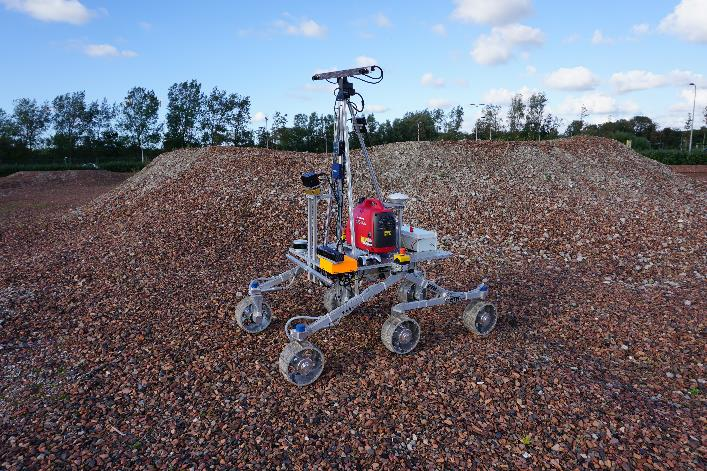
\includegraphics[scale=0.5]{hdpr_rover}
    \decoRule
    \caption[Heavy duty planetary rover]{
        The Heavy duty planetary rover (HDPR) \parencite{Boukas2016}.
    }
    \label{fig:hdpr_rover}
\end{figure}

\begin{itemize}
    \item Exteroceptive:
        \begin{itemize}
            \item LocCam stereo camera (PointGrey Bumblebee 2)
            \item PanCam stereo camera (PointGrey Grasshoper 2)
            \item Kinect time of flight camera
            \item MESA SR4500 time of flight camera
            \item Velodyne LiDAR (VLP-16)
        \end{itemize}
    \item Proprioceptive:
        \begin{itemize}
            \item Trimble GNSS receiver (BD970)
            \item Inertial Measurement Unit (Sensonor STIM300)
            \item Shaft Encoders and Potentiometers
        \end{itemize}
\end{itemize}

From these sensors, we exploit
\begin{enumerate*}[label=(\roman*)]
    \item the LocCam for visual odometry inputs and
    \item the PanCam for SLAM inputs.
\end{enumerate*}
The LocCam has a baseline of $\SI{120}{\mm}$, is positioned about
$\SI{1.1}{\m}$ above the ground and is tilted at an angle of $18^{\circ}$.
The PanCam has a baseline of $\SI{500}{\mm}$, is positioned about
$\SI{1.9}{\m}$ above the ground, is tilted at an angle of $19^{\circ}$ and
has a field of view (FoV) of $40^{\circ}$.

In addition, the Inertial Measurement Unit (IMU) provides measurements about
the orientation and acceleration of the robot.
Although the rest of the sensors are not actively used by our system,
they can be exploited for validation purposes.

\section{Overall System Architecture}

As we mentioned previously, the GA SLAM system was designed to function
with point cloud based inputs in addition to odometry inputs.

To utilize the sensor suite of the HDPR rover, we can extract point clouds
using stereo processing techniques and odometry estimation using visual
odometry methods.
For the former we employ the PanCam stereo camera and for the latter we make
use of the LocCam stereo camera.
Furthermore, we exploit the measurements received from the IMU to augment
the estimation of the robot's pose.
The utilization of each sensor of the HDPR rover w.r.t. to our system,
is shown in the system component diagram of Figure
\ref{fig:system_component_diagram}.

\begin{figure}[h!]
    \centering
    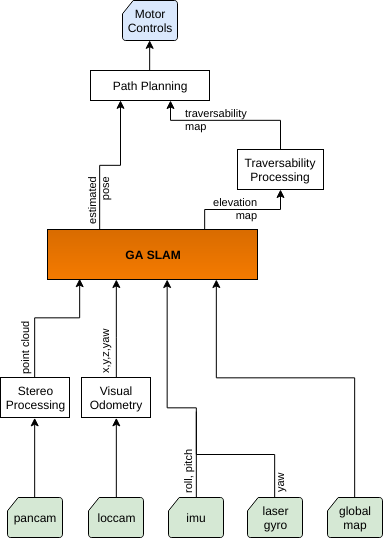
\includegraphics[scale=0.7]{system_component_diagram}
    \decoRule
    \caption[System component diagram]{
        The components of the system that enable the HDPR to perform
        autonomous navigation tasks.
    }
    \label{fig:system_component_diagram}
\end{figure}

As depicted, the local elevation map of the GA SLAM subsystem can be used
in order to extract a map that contains traversability features about the
surrounding environment of the rover, i.e. features that determine if
the rover is able to traverse a specific area.
At a next layer, the traversability map and the estimated pose from SLAM
can be utilized by a path planning module, with the aim to provide
autonomously control the rover in an unknown environment.
Finally, It should be noted that the choice of visual odometry
instead of plain wheel odometry, comes from the fact that a robot is prone
to slippage in outdoor environments, and more specifically planetary terrains.

\section{Robotic Software Framework}

The GA SLAM system \footnote{GA SLAM: \url{https://github.com/geromidg/GA_SLAM}}
was implemented as a framework-independent library for C++ and depends only
on libraries for linear algebra, point cloud processing and image processing.
However, with the aim to provide integration with the rest of HDPR's
software modules and tools, we developed a component to bridge
the library using the Robot Construction Toolkit (ROCK)
\footnote{ROCK: \url{https://www.rock-robotics.org}}.

ROCK is a software framework for the development of robotic systems,
similar to Robot Operating System (ROS).
It differs from ROS in the sense that the development of applications
is achieved using a model driven approach.
It is implemented on top of the Orocos Real-Time Toolkit (Orocos RTT)
component layer and can provide real-time capabilities to a system.
In addition, it contains a rich collection of reliable and extensible
modules that are ready to use as well as tools for visualization and
task monitoring.

In ROCK \parencite{Joyeux2011}, each distinct functionality of the system is
encapsulated in an RTT component (Figure \ref{fig:rock_component}) using a
tool called oroGen.
This tool, auto-generates the C++ code of the component, given
the specification of the component's interface.
The communication with the rest of the ROCK universe, is implemented through
a network of connected components.
This is achieved using the framework's Ruby modules which support the explicit
interconnection of a component's input port(s) with the output port(s)
of another component.

\begin{figure}[h!]
    \centering
    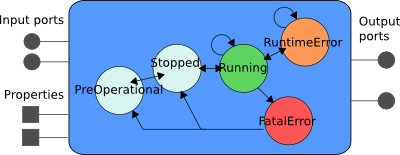
\includegraphics[scale=0.7]{rock_component}
    \decoRule
    \caption[ROCK component interface]{
        The interface and the state machine of a component in the Orocos
        Real-Time Toolkit. The output port(s) of a component can be explicitly
        connected to the input port(s) of another component. The properties
        are used to configure the component internally.
    }
    \label{fig:rock_component}
\end{figure}

\section{Orbiter Data Preprocessing}

As a means to validate the map matching capabilities of the system,
an orbiter (global) map is necessary.
A real example of such map has been reconstructed using orbital imagery,
depicted in Figure \ref{fig:hirise_map}, that was captured using the
High Resolution Imaging Science Experiment (HiRISE) camera mounted
on NASA's Mars Reconnaissance Orbiter (MRO) \parencite{Gallagher2005}.

It is possible to emulate an orbiter map using drone imagery.
The aerial images can then be used to reconstruct and provide a 3D
representation of the captured scene in the form of a densified point cloud.
At a later stage, the constructed point cloud can be projected in a 2D
grid and create an elevation map.

\begin{figure}[h!]
    \centering
    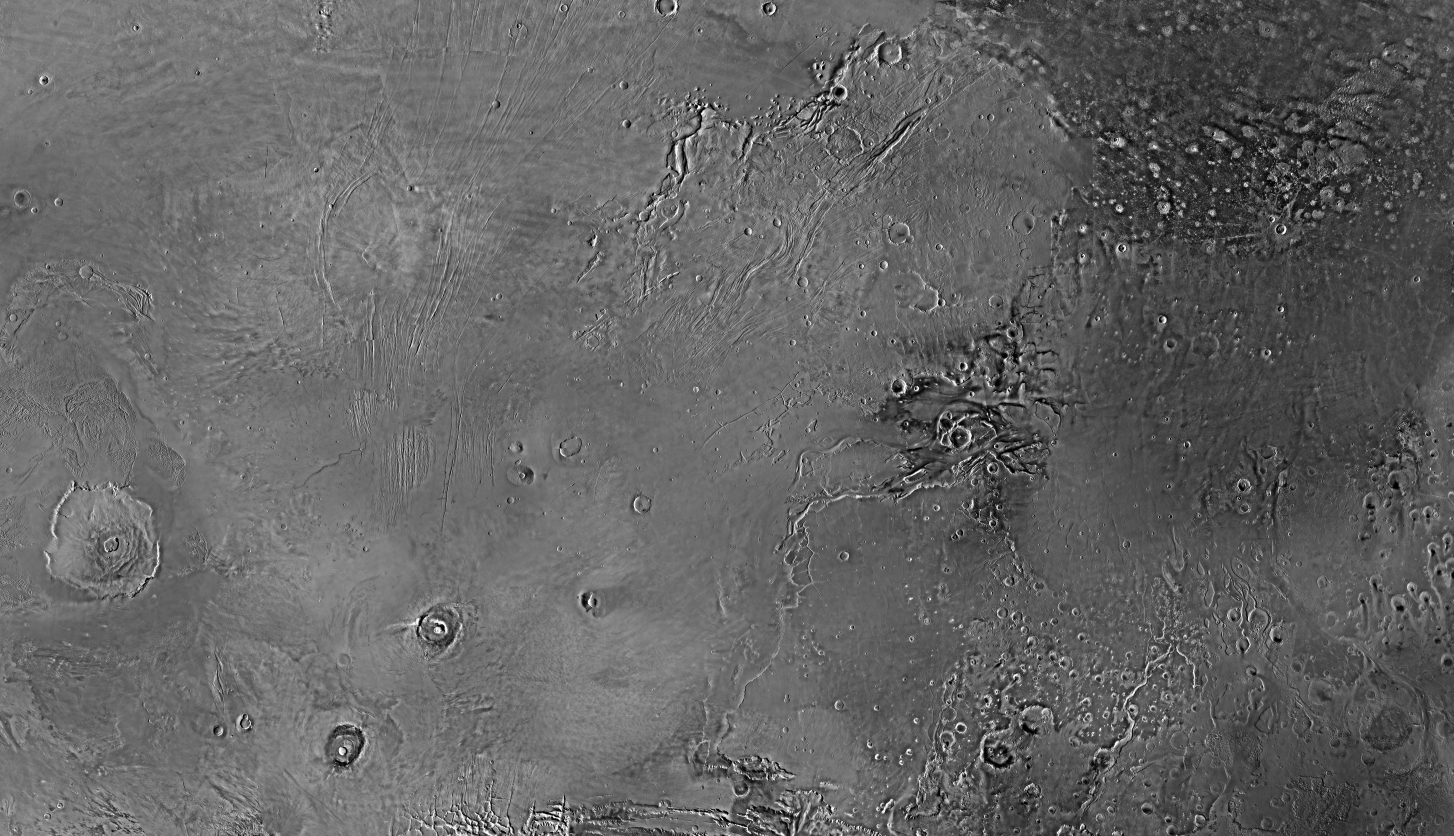
\includegraphics[scale=0.25]{hirise_map}
    \decoRule
    \caption[Mars view from HiRISE]{
        Close view of Mars that was captured using the HiRISE camera
        mounted on the Mars Reconnaissance Orbiter.
    }
    \label{fig:hirise_map}
\end{figure}

Prior to the projection, it is necessary to preprocess the global point cloud
in order to simplify it and transform it to a known reference system.
This is achieved in 4 steps:
\begin{enumerate*}[label=(\roman*)]
    \item voxelize point cloud to the desired resolution
    \item crop the voxel grid in the order of magnitude as the local map's
        size instead of using the whole information
        (e.g. for a local map of $\SI{10 x 10}{\m}$ crop the grid to
        $\SI{100 x 100}{\m}$)
    \item smooth the voxel grid using a Statistical Outlier Removal (SOR)
        filter which rejects points that are far from their neighbors
    \item transform the voxel grid to the robot's initial absolute pose.
\end{enumerate*}


%\label{Chapter4}

\chapter{Experimental Validation}

\section{Scope of Experiments}

Mention why mapping experiments are out of the scope\\
Explain briefly the purpose of the following experiments\\
Explain the type of the experiments

\begin{itemize}
    \item Purpose: validate the algorithm and its robustness in various terrains and configurations
    \item Type: SIL tests (precollected data)
\end{itemize}

\subsection{Environment}

Explain the environment of the collected data (location, traversed paths etc.)\\
Add figures showing the said environment/traverses

\subsection{Metrics}

Mention the metrics used

\begin{itemize}
    \item MSE of pose graph
    \item mean variance of pose graph,
    \item (execution times)
    \item etc.
\end{itemize}

\section{Experiments on Pose Estimation}

\subsection{Relative Localization Results}

Explain what the experiment is (test the accuracy of the particle filter)\\
Explain what is the expected accuracy of the estimation (1 cell size of local map)

\bigskip
\noindent
Add bird's eye view of XY plot comparing:
\begin{itemize}
    \item ground truth 2D position
    \item (Odometry)
    \item PF estimate
\end{itemize}

\noindent
Add plot showing the error vs the number of particles used\\
Add plot showing the mean variance of the estimate vs the number of particles used\\
Add table showing the execution time vs the numner of particles used\\
Add plot showing the error vs the resampling frequency

\bigskip
\noindent
Discuss the above results and what are the advantages/drawbacks while tuning each parameter

\section{Experiments on Global Map Matching}

\subsection{Absolute Localization Results}

Explain what the experiment is (test the drift correction on long range traverses)\\
Explain what is the expected accuracy of the correction (1 cell size of global map)

\bigskip
\noindent
Add bird's eye view of XY plot comparing:
\begin{itemize}
    \item ground truth 2D position
    \item (Odometry)
    \item PF estimate without global correction
    \item PF estimate with global correction
\end{itemize}

\bigskip
\noindent
Repeat test in environment with different distribution of features\\
(Repeat test in environment without features to show the limitation of the approach)

\bigskip
\noindent
Add table with the matching accuracy of the different experiments

\bigskip
\noindent
Discuss the threshold value that should be chosen on such environments

\subsection{Map Resolution Viability}

Explain what the experiment is (test under what resolutions can we expect a drift correction)

\bigskip
\noindent
Add figure showing local \& global maps with different resolution\\
Add table comparing global vs local map resolutions using the correction error (actual offset - matched location)

\bigskip
\noindent
Discuss the global and local map resolution of the current Mars missions and how these will change in the future (e.g. NASA is planning to have 0.25m orbiter map resolution by 2020)

 
%\label{Chapter5}

\chapter{Conclusion}

\section{Thesis Summary}

This thesis has considered the problem of perception for rovers that
aim to navigate autonomously in a planetary terrain.
We constructed an approach that is able to tackle the SLAM problem
in a relative context by making use of elevation mapping techniques using
3D point clouds and by employing a particle filter which utilizes a
scan matching method.
In addition, we extended the approach with the aim to correct errors
in position and orientation that accumulate over time using a template
matching method that locates the local elevation map in a globally referenced
one.

The proposed system was implemented as a standalone library and was
integrated with the software components of ESA's HDPR rover.
The integration with the HDPR's system was achieved using the ROCK
robotics framework.
This allowed the utilization of a rover with a sensor setup that bears close
resemblance to the one of the ExoMars mission.

Moreover, we demonstrated the developed system using collected data
from a Mars analogue (Chapter \ref{Chapter4}) and proved its
advantages and weaknesses in short and long range scenarios.
Specifically, the proposed method appeared to perform efficiently in
terrains that contained an average amount of elevation features (e.g. rocks).
However, in terrains that are characterized by the absence of such features,
the global pose correction mechanism fails to provide accurate matches.
Finally, we examined the influence the resolutions of the local and global
maps have on the matching technique.

\section{Contributions}

The main contribution of this thesis in terms of research,
is the development of a novel technique for minimizing the localization
drift with global map matching in addition to solving the SLAM problem
for a planetary rover.

For this purpose, we developed an open-source and research-oriented
C++ library with the following characteristics:

\begin{itemize}
    \item suitable for rough terrain navigation by utilizing
        2.5D (elevation) maps
    \item ability to correct the robot's global pose using map matching
        of local (robot-centric) and global (orbiter) elevation maps
    \item sensor-agnostic data registration using point clouds
        (enables the support for sensor such as lidar,
        stereo camera, ToF camera etc.)
    \item automatic sensor fusion when multiple point cloud inputs
        are provided without prior configuration
    \item adaptive design to fit the needs of different robots
        and applications.
\end{itemize}

\section{Directions for Future Extensions}

As we already mentioned, SLAM approaches on planetary rovers have an important
constraint which is the limited on board processing power.
Hence, it is important to design a lightweight system that requires as low
computations as possible.

With that in mind, a possible extension of the proposed particle filter
algorithm would be to model the space of the problem, i.e. localization,
in a discretized way instead of a continuous one.
This can be achieved by sampling particles in a 2D grid that has the same
resolution as the local map.
As a result, particles that fall in the same cell of the grid are eliminated
and are replaced by new particles.

Another direction for future work would be to exploit the uncertainty
of the robot's pose to improve the quality of the local map.
This can be accomplished using a neighborhood fusion method
\parencite{Fankhauser2014} by fusing nearby cells for each cell of the
map according to the variance of the robot's translation.
The variance values could be extracted directly from the particle filter,
by calculating the distribution of the particles, or by using the
motion model of the robot.

Finally, the global elevation map could be further utilized by using it
to initialize the cells of the local map.
This could provide a starting point for the fusion of new point cloud
data in the local map and increase the overall quality of the map.

\section{Applications}

Besides planetary scenarios, the proposed approach of this thesis
can also be used in Earth applications, with the obvious one being
autonomous driving vehicles.
Similarly to a planetary rover, self-driving cars require high
precision in terms of perception.

Although the usage of GPS data in such vehicles helps in the global
localization problem, its availability cannot be guaranteed at every
possible location, especially in non-urban areas.
A way to utilize the technique we developed in such applications,
would be to exploit global maps that have been a priori reconstructed
to contain information about the terrain's elevation.
This could provide self-driving vehicles with a mechanism to correct
possible drifts in position and orientation.

 

%----------------------------------------------------------------------------------------
%	THESIS CONTENT - APPENDICES
%----------------------------------------------------------------------------------------

%\appendix % Cue to tell LaTeX that the following "chapters" are Appendices

% Include the appendices of the thesis as separate files from the Appendices folder
% Uncomment the lines as you write the Appendices

%% Appendix A

\chapter{Frequently Asked Questions} % Main appendix title

\label{AppendixA} % For referencing this appendix elsewhere, use \ref{AppendixA}

\section{How do I change the colors of links?}

The color of links can be changed to your liking using:

{\small\verb!\hypersetup{urlcolor=red}!}, or

{\small\verb!\hypersetup{citecolor=green}!}, or

{\small\verb!\hypersetup{allcolor=blue}!}.

\noindent If you want to completely hide the links, you can use:

{\small\verb!\hypersetup{allcolors=.}!}, or even better: 

{\small\verb!\hypersetup{hidelinks}!}.

\noindent If you want to have obvious links in the PDF but not the printed text, use:

{\small\verb!\hypersetup{colorlinks=false}!}.

%\include{Appendices/AppendixB}
%\include{Appendices/AppendixC}

%----------------------------------------------------------------------------------------
%	BIBLIOGRAPHY
%----------------------------------------------------------------------------------------

\printbibliography[heading=bibintoc]

%----------------------------------------------------------------------------------------

\end{document}  
